% Created 2016-02-13 Sat 16:54
\documentclass[bigger]{beamer}
\usepackage[utf8]{inputenc}
\usepackage[T1]{fontenc}
\usepackage{fixltx2e}
\usepackage{graphicx}
\usepackage{longtable}
\usepackage{float}
\usepackage{wrapfig}
\usepackage{rotating}
\usepackage[normalem]{ulem}
\usepackage{amsmath}
\usepackage{textcomp}
\usepackage{marvosym}
\usepackage{wasysym}
\usepackage{amssymb}
\usepackage{hyperref}
\tolerance=1000
\usetheme{default}
\author{Nooreen S Dabbish}
\date{\textit{<2016-02-12 Fri>}}
\title{lassopart}
\hypersetup{
  pdfkeywords={},
  pdfsubject={},
  pdfcreator={Emacs 24.4.1 (Org mode 8.2.10)}}
\begin{document}

\maketitle
\begin{frame}{Outline}
\tableofcontents
\end{frame}



\section{Lasso Regression in (Casanova 2012)}
\label{sec-1}

\begin{frame}[label=sec-1-0-1]{Ensemble method based on lasso regression}
\begin{itemize}
\item takes advantage of lasso's sparsity property
\item index for scoring variable importance
\begin{itemize}
\item scores based on subsampling and ensemble learning
\item using penalized lasso linear regression
\end{itemize}
\item coordinate descent
\begin{itemize}
\item GLMNET library
\item time-efficient use of full data space
\end{itemize}
\item No feature reduction: full set of correlations
\end{itemize}
\end{frame}

\begin{frame}[fragile,label=sec-1-0-2]{Matrix vectorization and adding responses (gender)}
 \begin{verbatim}
 ## Create list of unique region abbreviations from original list
 ## Adds integers (starting with 2) to non-unique values
 setwd('~/Documents/BejingZhang')
 abbrev <- read.table("abbreviations.txt")
 abbrev[] <- lapply(abbrev, as.character)
 v <- vector("list", 0)
 v <- abbrev[[1]][1]
 for (j in 2:dim(abbrev)[1]){
     x <- 1
     y <- abbrev[[1]][j]
     while (is.element(y, v)){
        x <- x+1
        y <- paste0(abbrev[[1]][j],as.character(x), sep="")
     }
     v <- c(v,y)
 }

 table(v) # they are now all unique

 ## create list of downloaded folders with data
 ## there were problems reading in 954,955,956,957
 array <- c(787:839,841:851,853,857:865,867:872,875:878,
            880:938,940:953,974:978)
 array2 <-list()

metadata <- read.csv("metadata-bejingZangOnly.csv", header = TRUE)
head(metadata)
metadata <- metadata[,c("upload_data.id","upload_data.subject_pool", "upload_data.group_size")]
colnames(metadata) <- c("id","age","gender")
metadata[metadata$id == 787,]$gender

vectorgender <- data.frame(matrix(nrow=length(array), ncol=((length(v)*(length(v)-1)/2+1+1+1) )))


##need to create a vector of labels
corrlabels <- c()
for(i in 2:(length(v))){
    for (j in 1:(i-1)){
        corrlabels <- c(corrlabels,paste(v[i],v[j],sep="-"))
    }
}

colnames(vectorgender) <- c("id","age","gender",corrlabels)
levels(vectorgender$gender) <- c("Male","Female")

## Read in connectivity matrices, add row/col labels, and add 1 to diagonal
 for (i in 1:length(array)){
 array2[[i]] <- read.table(paste0(paste0("connectivity_matrix",as.character(array[i])),".txt"))
 dimnames(array2[[i]])[[1]] <- as.vector(v)
 dimnames(array2[[i]])[[2]] <- as.vector(v)
 array2[[i]] <- array2[[i]] + diag(x=1,nrow = length(array2[[i]]))
 vectorgender[i,] <- c(metadata[metadata$id == array[i], ]$id,
                       metadata[metadata$id == array[i], ]$age,
                       as.factor(metadata[metadata$id == array[i], ]$gender),
                       unlist(array2[[i]][upper.tri(array2[[i]],diag=FALSE)]))
 }


setwd('~/Dropbox/STAT 9190 Project/jstsp2015/Presentation2')
\end{verbatim}
\end{frame}


\subsection{Load GLMNET and fit data}
\label{sec-1-1}

\begin{frame}[fragile,label=sec-1-1-1]{Code}
 \begin{verbatim}
## install.packages("glmnet", repos='http://cran.us.r-project.org')
library(glmnet)

fit = glmnet(x = as.matrix(vectorgender[,-(1:3)]),
             y = as.vector(vectorgender$gender))

plot(fit, label =TRUE)
\end{verbatim}
\end{frame}

\begin{frame}[label=sec-1-1-2]{Plot}
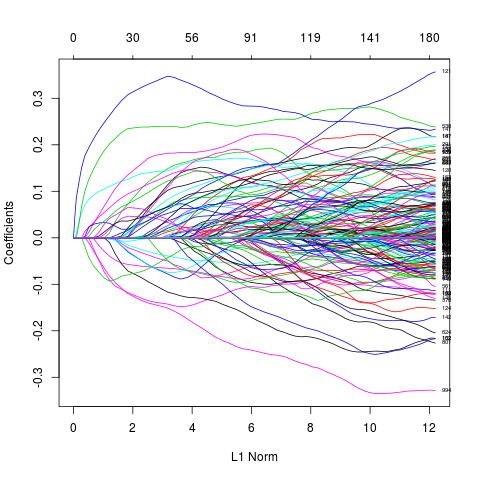
\includegraphics[width=.9\linewidth]{coeffplot.png}
\end{frame}

\subsection{Cross-Validation}
\label{sec-1-2}

\begin{frame}[fragile,label=sec-1-2-1]{Code}
 \begin{verbatim}
cvfit = cv.glmnet(x = as.matrix(vectorgender[,-(1:3)]),
                  y = (vectorgender$gender))

plot(cvfit)
\end{verbatim}
\end{frame}

\begin{frame}[label=sec-1-2-2]{Plot}
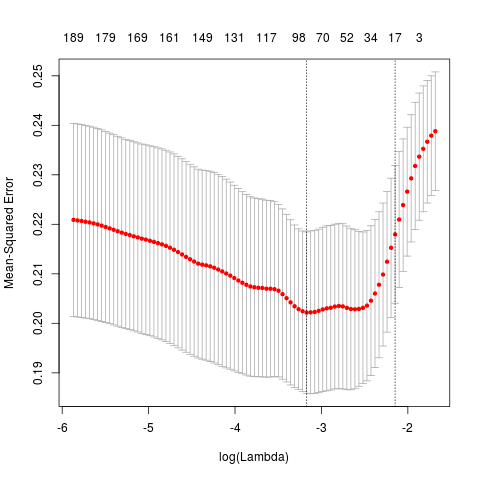
\includegraphics[width=.9\linewidth]{cvplot.png}
\end{frame}

\begin{frame}[fragile,label=sec-1-2-3]{Selected $\lambda$ s}
 \begin{verbatim}
cvfit$lambda.min
\end{verbatim}

\begin{verbatim}
[1] 0.07332683
\end{verbatim}

\begin{block}{\verb~lambda.min~ value that gives minimum cross-validated error}
\begin{verbatim}
cvfit$lambda.1se
\end{verbatim}

\begin{verbatim}
[1] 0.09252797
\end{verbatim}
\end{block}

\begin{block}{\verb~lambda.1se~ value that gives most regularized model with error vwithin one standard error of minimum cross-validated error}
\end{block}
\end{frame}
% Emacs 24.4.1 (Org mode 8.2.10)
\end{document}